% Mediator structural DAG (Supplement, Supp Fig 1), TikZ standalone.
% Split out of the former dual mediator+confounder figure so each renders full size.
% Body composition is a MEDIATOR (dsc -> fatlean); fatlean observed/white.
% Build (fontspec + Inter -> xelatex; run TWICE). In a sandboxed shell:
%   TEXMFVAR=$TMPDIR/texmf-var TEXMFCACHE=$TMPDIR/texmf-cache xelatex mediator.tex
% Output: mediator.pdf -> outputs/figures/final/supp-fig-1-mediator-dag.pdf

\documentclass[border=10pt]{standalone}
\usepackage{fontspec}
\setsansfont{Inter}
\renewcommand{\familydefault}{\sfdefault}
\usepackage{tikz}
\usetikzlibrary{arrows.meta, positioning, fit, backgrounds, calc}

\definecolor{stageSetup}{HTML}{CFD8EA}
\definecolor{stageLang}{HTML}{CFDFCD}
\definecolor{stageAuth}{HTML}{E3C2BC}
\definecolor{stageOut}{HTML}{D9D9D9}
\definecolor{dark}{HTML}{1E293B}
\definecolor{slate}{HTML}{64748B}
\definecolor{linegreen}{HTML}{3F7E4E}
\definecolor{linered}{HTML}{A85D52}
\definecolor{lineamber}{HTML}{C77B30}

\tikzset{
  font=\sffamily\footnotesize,
  exposure/.style={rectangle, rounded corners=4pt, draw=slate!75, line width=0.7pt,
                   fill=stageLang, text=dark, align=center,
                   minimum width=1.8cm, minimum height=0.95cm},
  outcome/.style={rectangle, rounded corners=4pt, draw=slate!75, line width=0.7pt,
                  fill=stageSetup, text=dark, align=center,
                  minimum width=1.6cm, minimum height=0.95cm},
  msas/.style={rectangle, rounded corners=4pt, draw=linered, line width=0.9pt,
               fill=stageAuth, text=dark, align=center,
               minimum width=1.5cm, minimum height=0.95cm},
  obs/.style={rectangle, rounded corners=4pt, draw=slate!75, line width=0.7pt,
              fill=white, text=dark, align=center,
              minimum width=1.5cm, minimum height=0.85cm},
  latent/.style={rectangle, rounded corners=4pt, draw=slate!85, line width=0.7pt, dashed,
                 fill=stageOut, text=dark, align=center,
                 minimum width=1.7cm, minimum height=0.95cm},
  causal/.style={-{Latex[length=2.6mm]}, draw=linegreen, line width=1.4pt},
  conf/.style={-{Latex[length=2.6mm]}, draw=linered, line width=1.0pt},
  latentedge/.style={-{Latex[length=2.6mm]}, draw=lineamber, line width=1.0pt, dashed},
  other/.style={-{Latex[length=2.6mm]}, draw=slate, line width=0.6pt, opacity=0.85},
  anno/.style={font=\sffamily\itshape\small, text=slate},
}

\begin{document}
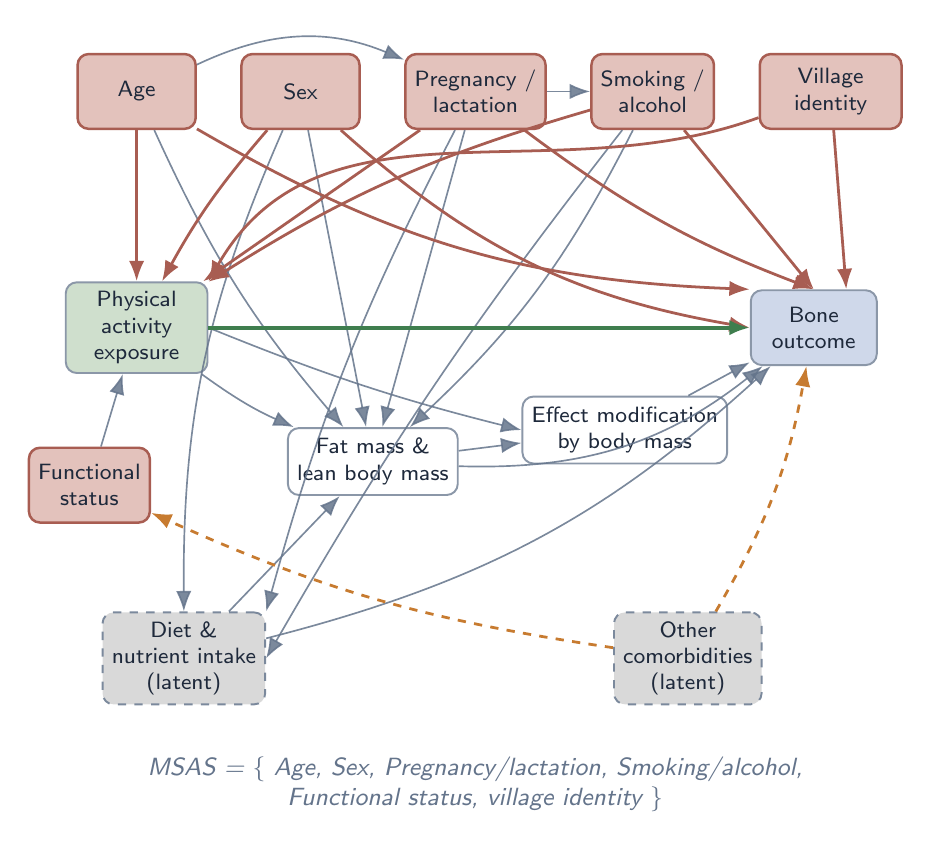
\begin{tikzpicture}

% #1 = x-offset (0 here), #2 = fatlean style (obs), #3 = body-comp edge key (med)
\newcommand{\drawpanel}[3]{%
  \begin{scope}[xshift=#1 cm]
    \node[msas]     (age)  at (0.0, 6.2) {Age};
    \node[msas, right=0.55cm of age] (sex)  {Sex};
    \node[msas, right=0.55cm of sex] (pl)   {Pregnancy /\\ lactation};
    \node[msas, right=0.55cm of pl]  (smk)  {Smoking /\\ alcohol};
    \node[msas, minimum width=1.8cm, right=0.55cm of smk] (vill) {Village\\ identity};

    \node[exposure] (dsc)  at (0.0, 3.2) {Physical\\ activity\\ exposure};
    \node[outcome]  (osteo) at (8.6, 3.2) {Bone\\ outcome};
    \node[obs]      (em)   at (6.2, 1.9) {Effect modification\\ by body mass};
    \node[#2]       (fl)   at (3.0, 1.5) {Fat mass \&\\ lean body mass};

    \node[msas]     (fs)   at (-0.6, 1.2) {Functional\\ status};
    \node[latent]   (diet) at (0.6, -1.0) {Diet \&\\ nutrient intake\\ (latent)};
    \node[latent]   (comorb) at (7.0, -1.0) {Other\\ comorbidities\\ (latent)};

    % --- grey "other" edges ---
    \draw[other] (age) to[bend left=24] (pl);
    \draw[other] (pl)  -- (smk);
    \draw[other] (age) to[bend right=8] (fl);
    \draw[other] (sex) -- (fl);
    \draw[other] (pl)  -- (fl);
    \draw[other] (smk) to[bend left=10] (fl);
    \draw[other] (sex) to[bend right=12] (diet.north);
    \draw[other] (pl)  to[bend right=6]  (diet.north east);
    \draw[other] (smk) to[bend right=4]  (diet.east);
    \draw[other] (dsc.east) to[bend right=4] (em.west);
    \draw[other] (fl)  to[bend right=20] (osteo);
    \draw[other] (fl)  -- (em);
    \draw[other] (em)  -- (osteo);
    \draw[other] (diet) to[bend right=14] (osteo);
    \draw[other] (diet) -- (fl);
    \draw[other] (fs)  -- (dsc);
    \ifnum\pdfstrcmp{#3}{med}=0
      \draw[other] (dsc) to[bend right=6] (fl);
    \else
      \draw[other] (fl) to[bend left=6]  (dsc);
    \fi

    % --- red confounder edges: {age,sex,pl,smk,vill} -> {dsc,osteo} ---
    \draw[conf] (age) -- (dsc);
    \draw[conf] (age) to[bend right=14] (osteo.north west);
    \draw[conf] (sex) to[bend right=6] (dsc);
    \draw[conf] (sex) to[bend right=16] (osteo.west);
    \draw[conf] (pl)  -- (dsc);
    \draw[conf] (pl)  to[bend right=8] (osteo.north);
    \draw[conf] (smk) to[bend right=8] (dsc);
    \draw[conf] (smk) -- (osteo.north);
    \draw[conf] (vill) to[out=200,in=60] (dsc.north east);
    \draw[conf] (vill) -- ([xshift=-4mm]osteo.north east);

    % --- amber dashed latent edges ---
    \draw[latentedge] (comorb) to[bend left=8]  (fs);
    \draw[latentedge] (comorb) to[bend right=10] (osteo);

    % --- green causal edge (drawn last) ---
    \draw[causal] (dsc) -- (osteo);
  \end{scope}
}

\drawpanel{0}{obs}{med}

\node[anno, align=center] at (4.3, -2.6)
  {MSAS = \{ Age, Sex, Pregnancy/lactation, Smoking/alcohol,\\ Functional status, village identity \}};

\end{tikzpicture}
\end{document}
